\documentclass[aspectratio=169,11pt]{beamer}

% ============================================================
% SISMID 2026 -- Day 1, 11:00 session
% Part 1: Dengue exercise (S. Yang + C. Djorno)
% Intro to Google Dengue Trends -> visualize -> least squares ->
% map search onto dengue activity -> stretch (dynamic + Lasso).
% Agent-driven throughout.
% Compile: pdflatex dengue-exercise.tex  (run twice)
% ============================================================

\IfFileExists{beamerthememetropolis.sty}{
  \usetheme{metropolis}
  \metroset{progressbar=frametitle, sectionpage=progressbar, numbering=fraction}
}{
  \usetheme{Boadilla}
  \usecolortheme{seahorse}
  \setbeamertemplate{navigation symbols}{}
}

\usepackage[utf8]{inputenc}
\usepackage[T1]{fontenc}
\usepackage{tikz}
\usetikzlibrary{arrows.meta, positioning, fit, backgrounds, calc}
\usepackage{xcolor}
\usepackage{listings}
\usepackage{amsmath}

\definecolor{AccentA}{HTML}{2A6F97}
\definecolor{AccentB}{HTML}{C1666B}
\definecolor{AccentC}{HTML}{3B8A5B}
\setbeamercolor{frametitle}{bg=AccentA}
\setbeamercolor{progress bar}{fg=AccentB}

\definecolor{skbg}{rgb}{0.96,0.96,0.94}
\lstdefinestyle{prompt}{
  basicstyle=\ttfamily\scriptsize,
  backgroundcolor=\color{skbg},
  showstringspaces=false, breaklines=true,
  frame=single, framesep=4pt, columns=fullflexible, numbers=none,
}
\lstset{style=prompt}

\tikzset{
  cbox/.style={draw=AccentA, very thick, rounded corners, align=center,
    minimum height=1.0cm, inner sep=6pt, font=\small, fill=AccentA!6},
  sbox/.style={draw=AccentA, thick, rounded corners, align=center,
    minimum height=0.85cm, inner sep=4pt, font=\scriptsize, fill=AccentA!6},
  rbox/.style={draw=AccentB, thick, rounded corners, align=center,
    minimum height=0.85cm, inner sep=4pt, font=\scriptsize, fill=AccentB!8},
  gbox/.style={draw=AccentC, thick, rounded corners, align=center,
    minimum height=0.85cm, inner sep=4pt, font=\scriptsize, fill=AccentC!8},
  flow/.style={-{Stealth[length=3mm]}, very thick, draw=AccentB},
  flowq/.style={-{Stealth[length=2.4mm]}, thick, draw=AccentA!70},
}

% flow cues for the instructor: where to hand off between slides, sheet, notebook
\newcommand{\tonb}[1]{\vspace{0.1em}\begin{flushright}\footnotesize\textcolor{AccentB}{$\blacktriangleright$~\textbf{#1}}\end{flushright}}
\newcommand{\toslides}[1]{\vspace{0.1em}\begin{flushright}\footnotesize\textcolor{AccentC}{$\blacktriangleleft$~\textbf{#1}}\end{flushright}}

\title{The Dengue Exercise}
\subtitle{Map a search signal onto disease activity, with an agent}
\author{Shihao Yang \quad\textbullet\quad Candice Djorno}
\institute{SISMID 2026 \textbullet\ Day 1, 11:00}
\date{July 20, 2026}

\begin{document}

\begin{frame}
  \titlepage
\end{frame}

\begin{frame}{Where we are}
  An hour ago you \textbf{scraped} dengue search interest for Mexico. Now the real
  question:
  \begin{block}{Does a search signal actually track the disease?}
    We will build a tiny \textbf{Google Dengue Trends}: fit search onto reported cases on
    the early years, then predict the later years and see how well it holds up.
  \end{block}
  \vspace{0.4em}
  \begin{itemize}
    \item Same two lanes as this morning: \textbf{Lane A} prompt an agent (Codex, Claude
          Code, Antigravity CLI) with \texttt{notebooks/dengue\_exercise.ipynb};
          \textbf{Lane B} the pre-filled \texttt{notebooks/dengue\_exercise\_soln.ipynb}.
    \item You will paste \emph{one prompt per step} and keep the judgment.
  \end{itemize}
\end{frame}

\begin{frame}{Roadmap}
  \tableofcontents
\end{frame}

\begin{frame}{How this hour runs (for the instructor)}
  You move among three things; the slides cue every hand-off.
  \begin{center}
  \resizebox{0.95\textwidth}{!}{%
  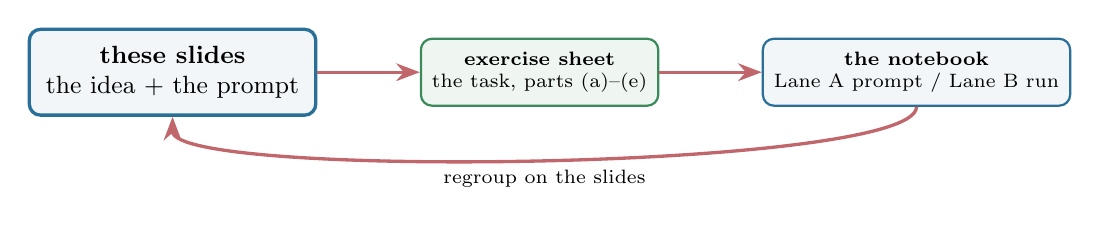
\begin{tikzpicture}[node distance=0.6cm and 1.3cm]
    \node[cbox] (sl) {\textbf{these slides}\\the idea + the prompt};
    \node[gbox, right=of sl] (sh) {\textbf{exercise sheet}\\the task, parts (a)--(e)};
    \node[sbox, right=of sh] (nb) {\textbf{the notebook}\\Lane A prompt / Lane B run};
    \draw[flow] (sl) -- (sh); \draw[flow] (sh) -- (nb);
    \draw[flow] (nb.south) .. controls +(0,-0.8) and +(0,-0.8) ..
      node[below,font=\scriptsize]{regroup on the slides} (sl.south);
  \end{tikzpicture}}
  \end{center}
  \begin{itemize}
    \item \textbf{Hand out now:} \texttt{exercise/dengue-exercise-2026.pdf} (the task, a--e).
    \item \textbf{Open now:} \texttt{notebooks/dengue\_exercise.ipynb} (Lane A) or
          \texttt{...\_soln.ipynb} (Lane B).
    \item Follow the \textcolor{AccentB}{$\blacktriangleright$ to the notebook} and
          \textcolor{AccentC}{$\blacktriangleleft$ back to slides} cues at the corners.
  \end{itemize}
\end{frame}

% ===============================================================
\section{Intro to Google Dengue Trends}

\begin{frame}{The idea behind Google Dengue Trends}
  When dengue rises, people search: \emph{dengue}, \emph{sintomas de dengue},
  \emph{mosquito}.
  \begin{itemize}
    \item Aggregate search volume moves \textbf{with} disease activity, and it is
          available \textbf{cheaply and in near-real-time}, ahead of official case counts.
    \item This is the digital-epidemiology origin story: \textbf{Google Flu Trends}
          (2009) nowcast influenza from searches; the same recipe was tried for dengue in
          tropical countries.
  \end{itemize}
  \vspace{0.3em}
  \begin{center}
    \itshape The whole field starts from one plot: a search curve and a disease curve
    that rise and fall together.
  \end{center}
\end{frame}

\begin{frame}{The data}
  \texttt{MX\_Dengue\_trends.csv} (Mexico, monthly, 2004--2011):
  \begin{itemize}
    \item \texttt{Dengue CDC} --- reported dengue \textbf{cases} (Mexican Ministry of
          Health). This is the \textbf{ground truth} we try to match.
    \item \texttt{dengue}, \texttt{sintomas de dengue}, \texttt{mosquito},
          \texttt{dengue sintomas} --- Google \textbf{search} interest, the same kind of
          series you scraped this morning.
  \end{itemize}
  \vspace{0.3em}
  \begin{center}
  \resizebox{0.8\textwidth}{!}{%
  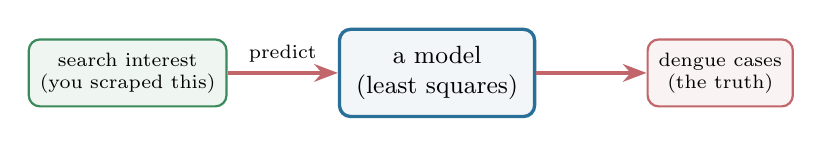
\begin{tikzpicture}[node distance=1.4cm]
    \node[gbox] (s) {search interest\\(you scraped this)};
    \node[cbox, right=of s] (m) {a model\\(least squares)};
    \node[rbox, right=of m] (y) {dengue cases\\(the truth)};
    \draw[flow] (s) -- node[above,font=\scriptsize]{predict} (m);
    \draw[flow] (m) -- (y);
  \end{tikzpicture}}
  \end{center}
  \vspace{0.2em}
  \begin{center}
    \itshape Exercise sheet: \texttt{exercise/dengue-exercise-2026.pdf}.
  \end{center}
\end{frame}

\begin{frame}{The task in one line}
  \begin{block}{Goal}
    Fit \textbf{search $\rightarrow$ cases} on 2004--2006, then use that line to
    \textbf{predict} cases for 2007--2011 from search alone, and judge how well a cheap
    search signal stands in for slow case reports.
  \end{block}
  \vspace{0.5em}
  Five parts (from the exercise sheet):
  \begin{enumerate}
    \item plot cases over time,
    \item fit a least-squares line on the training years,
    \item show the fit on the training years,
    \item predict and check the validation years,
    \item discuss: how would you improve it?
  \end{enumerate}
  \tonb{Hand out the sheet, open the notebook; the next slides are the prompts, one per step.}
\end{frame}

% ===============================================================
\section{Doing it with an agent}

\begin{frame}{Agent-first, one prompt per step}
  You will not hand-write pandas. You describe each step and its check; the agent writes
  and runs the code.
  \begin{center}
  \resizebox{0.8\textwidth}{!}{%
  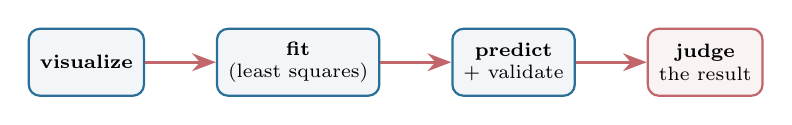
\begin{tikzpicture}[node distance=0.9cm]
    \node[sbox] (a) {\textbf{visualize}};
    \node[sbox, right=of a] (b) {\textbf{fit}\\(least squares)};
    \node[sbox, right=of b] (c) {\textbf{predict}\\+ validate};
    \node[rbox, right=of c] (d) {\textbf{judge}\\the result};
    \draw[flow] (a) -- (b); \draw[flow] (b) -- (c); \draw[flow] (c) -- (d);
  \end{tikzpicture}}
  \end{center}
  \vspace{0.3em}
  \begin{center}
    \itshape Lane B has the same steps pre-run, so a stuck neighbor is never blocked.
  \end{center}
\end{frame}

\begin{frame}[fragile]{Step 1: visualize (look before you model)}
  \begin{block}{Prompt (paste this)}
  \begin{lstlisting}
Load MX_Dengue_trends.csv. "Dengue CDC" is monthly dengue
cases in Mexico; "dengue" is Google search interest. Plot
the cases over time. Then overlay the "dengue" search
series on a second y-axis, and print the correlation
between the two columns.
  \end{lstlisting}
  \end{block}
  \begin{itemize}
    \item You are checking three things: do they \textbf{move together}? is there a
          \textbf{lead or lag}? any \textbf{gaps or spikes} that will fool a model?
    \item If the two curves clearly track each other, a straight line already has a chance.
  \end{itemize}
\end{frame}

\begin{frame}[fragile]{Step 2: least squares, the honest baseline}
  Let $y_t$ be dengue cases and $x_t$ the \texttt{dengue} search volume. Fit on
  2004--2006:
  \[
    y_t = a + b\,x_t + \varepsilon_t,\qquad
    (\hat a,\hat b)=\arg\min_{a,b}\sum_{t}\bigl(y_t-a-b\,x_t\bigr)^2 .
  \]
  \begin{block}{Prompt (paste this)}
  \begin{lstlisting}
Using only the first 36 months (2004-2006) as training,
fit ordinary least squares: Dengue CDC ~ dengue. Report the
intercept and slope, the in-sample R^2, and overlay the
fitted line on a scatter of cases vs search.
  \end{lstlisting}
  \end{block}
  \begin{center}
    \itshape One search term, one slope. This is Google Dengue Trends stripped to its core.
  \end{center}
\end{frame}

\begin{frame}[fragile]{Step 3: predict, then judge out of sample}
  In-sample fit always looks good. What matters is the years the line has \emph{not} seen.
  \begin{block}{Prompt (paste this)}
  \begin{lstlisting}
Using the intercept and slope from training, predict dengue
cases for 2007-2011 from the "dengue" search column alone.
Plot predicted vs actual cases over time, and report the
out-of-sample correlation and RMSE. Do NOT refit on 2007+.
  \end{lstlisting}
  \end{block}
  \begin{itemize}
    \item Report out-of-sample error, not just $R^2$. That gap is the lesson.
    \item \textbf{Your check:} the last training point is 2006, and nothing after 2006
          touched the fit. Agents sometimes leak the future; catch it.
  \end{itemize}
  \toslides{Once everyone has run the three steps, back to the slides to check the work.}
\end{frame}

\begin{frame}{Verify what the agent produced}
  Before you trust a number, run one plot and one question:
  \begin{itemize}
    \item \textbf{Split is honest:} training ends 2006, prediction uses only search.
    \item \textbf{Scales and axes:} predicted cases in a plausible range, dates aligned.
    \item \textbf{Face validity:} do predicted peaks land in the right seasons?
    \item \textbf{Reproducible:} rerun; the fit should not wander.
  \end{itemize}
  \vspace{0.3em}
  \begin{alertblock}{The habit}
    The agent is fast, not infallible. Every output earns one sanity check before it
    counts. That is the skill this exercise builds.
  \end{alertblock}
\end{frame}

\begin{frame}{Step 4: a good fit is not a correct model}
  \begin{itemize}
    \item A single search term can track a disease for a while because both track the
          \textbf{season}, then break when behavior changes.
    \item \textbf{Google Flu Trends} is the famous cautionary tale: it beat lagged CDC
          data for years, then badly overshot as media coverage and the search algorithm
          shifted.
  \end{itemize}
  \vspace{0.3em}
  \begin{alertblock}{Identifiability}
    Fitting well does not prove the mechanism is right. Validate out of sample, re-check
    every season, and stay humble about what a correlation means.
  \end{alertblock}
  \begin{center}
    \itshape This is exactly why tomorrow's ARGO adds the disease's own history and
    refits as it goes.
  \end{center}
\end{frame}

% ===============================================================
\section{Stretch: dynamic training and Lasso}

\begin{frame}[fragile]{If you finished early: a dynamic model with Lasso}
  Stretch task on the \texttt{sarahhbellum/Zika-tutorial} data.
  \begin{block}{Prompt (paste this)}
  \begin{lstlisting}
Using the Zika tutorial data, fit the search-to-cases model
with DYNAMIC training: refit on a rolling 2-year window
instead of once. With several search terms, use Lasso (L1)
so useless terms drop out. Compare its out-of-sample error
to the single-term static line from before.
  \end{lstlisting}
  \end{block}
  \[
    \min_{a,\,\boldsymbol\beta}\ \sum_t\Bigl(y_t-a-\textstyle\sum_j \beta_j x_{j,t}\Bigr)^2
    \;+\; \lambda\sum_j |\beta_j| .
  \]
  \tonb{Stretch runs in the notebook too; autoregression itself waits for ARGO on Day 2.}
\end{frame}

\begin{frame}{Why these two upgrades}
  \begin{columns}[T]
    \begin{column}{0.5\textwidth}
      \textbf{Dynamic training}
      \begin{itemize}
        \item refit on a rolling window
        \item adapts as the search-disease link drifts
        \item the fix Google Flu Trends lacked
      \end{itemize}
    \end{column}
    \begin{column}{0.5\textwidth}
      \textbf{Lasso ($\ell_1$)}
      \begin{itemize}
        \item many candidate search terms in
        \item only the useful ones survive
        \item exactly what you want from a scraped pile of queries
      \end{itemize}
    \end{column}
  \end{columns}
  \vfill
  \begin{center}
    \itshape Dynamic training plus term selection is the on-ramp to ARGO on Day 2.
  \end{center}
\end{frame}

% ===============================================================
\section{Wrap-up}

\begin{frame}{What you built}
  \begin{itemize}
    \item A working \textbf{mini Google Dengue Trends}: a search signal mapped onto dengue
          activity in Mexico, fit on the past and \textbf{honestly validated} on the future.
    \item You did it by \textbf{describing steps to an agent} and checking its work, not by
          memorizing pandas.
    \item You saw the field's core warning first-hand: a great fit can still be a poor
          forecast.
  \end{itemize}
  \vspace{0.3em}
  \begin{center}
    \itshape The same loop (visualize, fit, predict, judge) is every model you will build
    this week.
  \end{center}
\end{frame}

\begin{frame}{Looking ahead: from this line to ARGO}
  \begin{itemize}
    \item \textbf{This afternoon:} Google Trends in depth, why the same pull returns
          different numbers, and how preprocessing restores its forecasting power.
    \item \textbf{Day 2:} turn this one-term line into \textbf{ARGO}: add the disease's own
          recent history (autoregression), many selected terms, and dynamic training.
  \end{itemize}
  \vfill
  \begin{center}
    \itshape You now have the baseline the rest of the course improves on.
  \end{center}
\end{frame}

\begin{frame}[standout]
  Questions?\\[0.4em]
  \small Sheet: \texttt{exercise/dengue-exercise-2026.pdf} \quad\textbullet\quad
  Notebook: \texttt{notebooks/dengue\_exercise(\_soln).ipynb}
\end{frame}

\end{document}
